\chapter{Computational Geometry}
In this chapter, we present some of the Computational Geometry notion about mesh and Delaunay triangulation useful to full understand the reconstruction method described in the thesis. 
\section{Manifold Surfaces in \texorpdfstring{$\mathbb{R}^n$}{}}
We give the basis to formulate a formal definition of 2-manifold mesh, since the reconstruction algorithm we propose deals with these type of surfaces. 
\subsection{Topological Space}
A 2-manifold surface is particular specialization of topological space. 
A topological space is usually a set of points together with a  relationship defining a set of neighbors of each points. More formally:
\begin{mydef}
\textbf{Topological Space}

  Given a set $X$ and a set of subsets $\tau$, named open sets; $(X, \tau)$ is a topological space if:
  \begin{itemize}
    \item $\emptyset \in \tau$;
    \item $X \in \tau$;
    \item $\forall t_1,t_2 \in \tau $, $t_1 \cup t_2 \in \tau$;
    \item the intersection of any finite number of subsets in $\tau$.
  \end{itemize}
\end{mydef}
The set $\tau$ is named topology.
For each set $X$ is always possible to define two topologies: the indiscrete or trivial topology, consisting of $X$ and $\emptyset$; the discrete topology, containing all of the possible subsets of $X$.

Other examples of topological spaces are metrical spaces. 
\begin{mydef}
  \textbf{Metrical Space}
  
A metrical space is a pair $(M, d)$, where $M$ is a set of points, and $d$ is a metric on $M$ such that, for any $x$, $y$ and $z \in M$:
\begin{itemize}
  \item $d(x, y) \geq 0$
  \item $d(x, y) = 0 \Longleftrightarrow x = y$
  \item $d(x, y) = d(y, x)$
  \item $d(x, z) \leq d(x, y) + d(y, z)$
\end{itemize}

\end{mydef}


Whenever $M = \mathbb{R}^k$ and $d$ is the Euclidean distance, then, $(\mathbb{R}^k, d)$ is the Euclidean topological space; in the case of 3D reconstruction, $k=3$.
The set of subset $\tau$ defining a topology in this case is composed by all the open balls
\[
B_k(x_0, r) = \{x \\in \mathbb{R}^k | d(x_0, x) < r\}
\]
with $x_0 \in M$ and $r > 0$.
To define a 2-manifold and we need the notion of homeomorphism.

\begin{mydef}
   \textbf{Homeomorphism}
   
   Given two topological spaces $(M_1, d_1)$ and $(M_2, d_2)$, a homeomorphism is a function $f:M_1\longrightarrow M_2$, such that:
   \begin{itemize}
    \item $f$ is bijective;
    \item $f$ is continuous;
    \item $f{-1}$ is continuous.
   \end{itemize}
\end{mydef}

For instance, the open interval $(a, b)$ is homeomorphic to $\mathbb{R}$ for any $a < b$; and $B_k(\mathbf{0}, 1)$ is homeomorphic to $\mathbb{R}^k$. 

\subsection{\texorpdfstring{$k$}-manifold}
A $k$-manifold, with $k \in \mathbb{N}$ is a topological space that is locally similar to $\mathbb{R}^k$. More formally:

\begin{mydef}
 \textbf{$k$-manifold in $\mathbb{R}^n$}
 
 Given $M \subseteq \mathbb{R}$ and $1 < k < n, k \in \mathbb{R}$, them, $(M, \tau_M)$ is a $k$-manifold if $\forall \mathbf{x} \in M$, then $\mathbf{x} \in V$ and $V$ is homeomorphic to $B_k(\mathbf{0}, 1)$.
\end{mydef}

In the thesis we deal with 2-manifolds in $\mathbb{R}^3$, named surfaces, in particular with connected surfaces. 

\begin{mydef}
\textbf{Connected Space}

A topological space is connected if it cannot be represented as the union of two disjoint nonempty open sets. 
\end{mydef}

Every 2-manifold can be categorized according to its genus. Intuitively, the genus is the number of holes in the surface. Formally


 
\begin{mydef}
\textbf{Genus}

Given a connected surface $M$, its genus is an integer number $h$ equals to the maximum number of cuts along non intersecting curves such that the resulting surfaces keeps the connected property.
\end{mydef}

In Figure \ref{fig:torus} we show examples of different genus surfaces: the sphere has no holes, so its genus is 0, the torus has one ``hole`` and its genus is 1, double torus and triple torus has respectively two and three holes therefore their genus is 2 and 3.
\begin{figure}

 \begin{tabular}{cccc}
  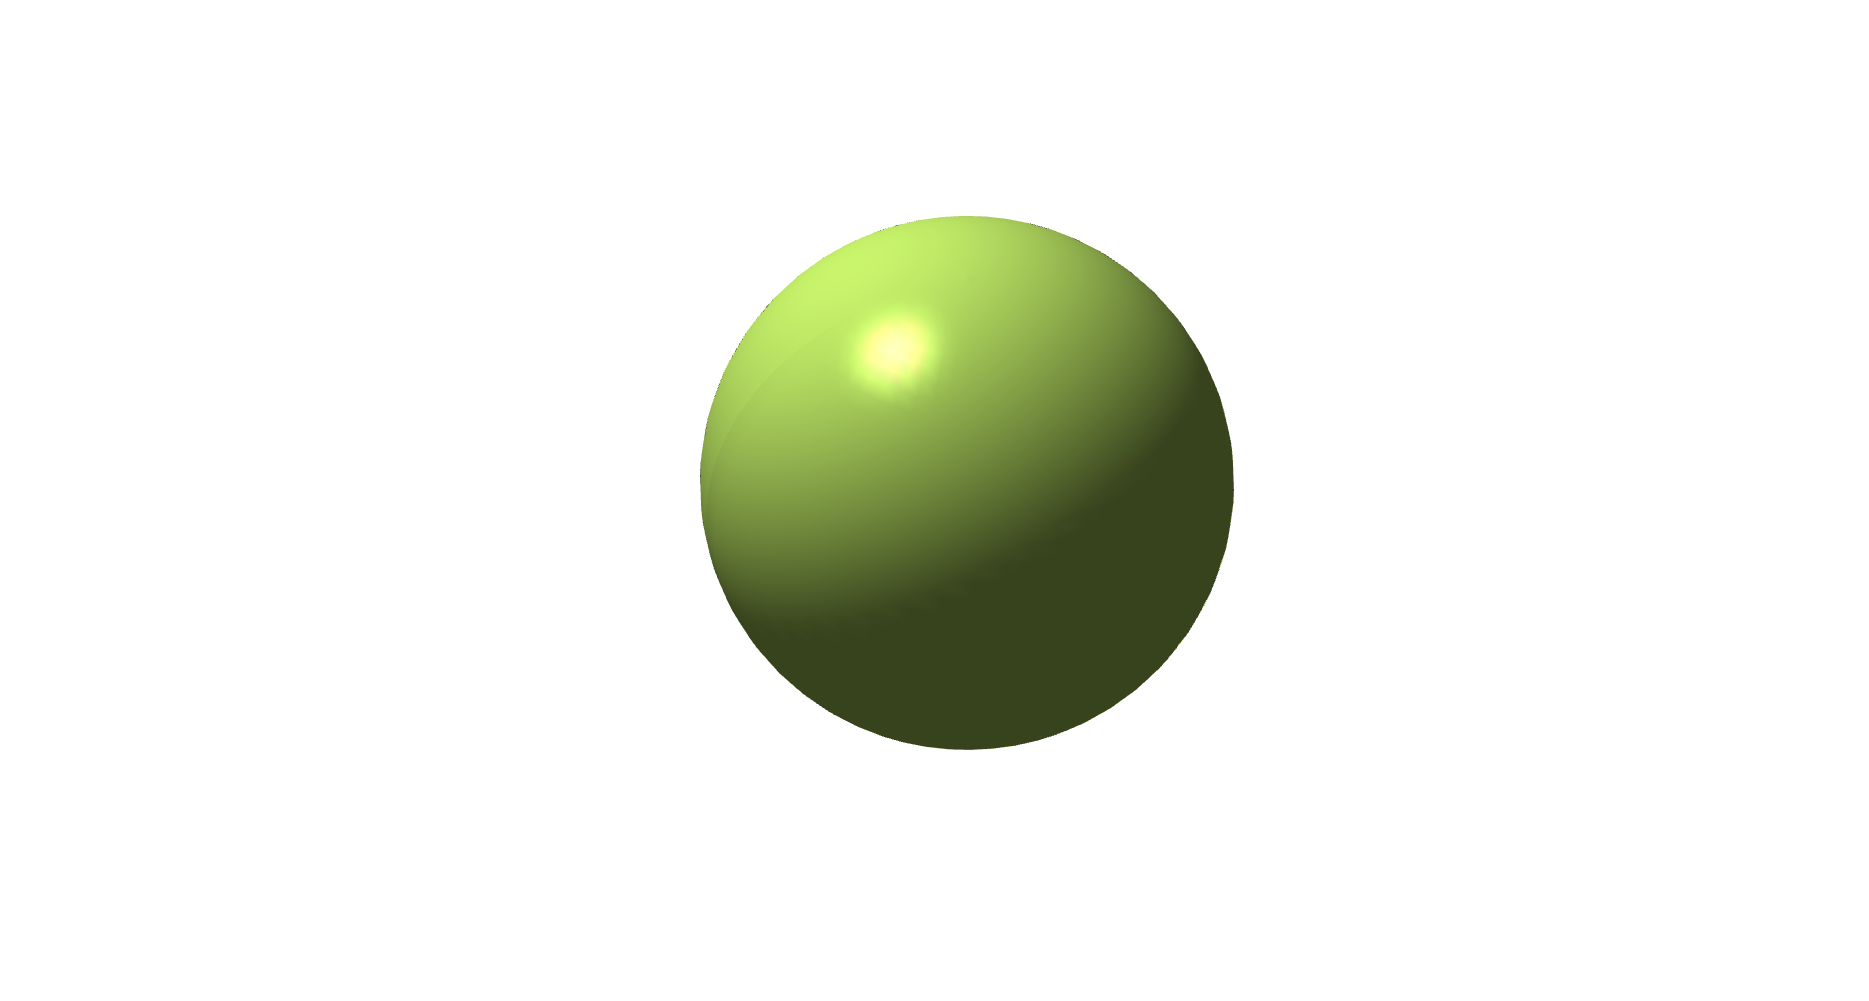
\includegraphics[width=0.21\columnwidth]{./img/sphere}&
  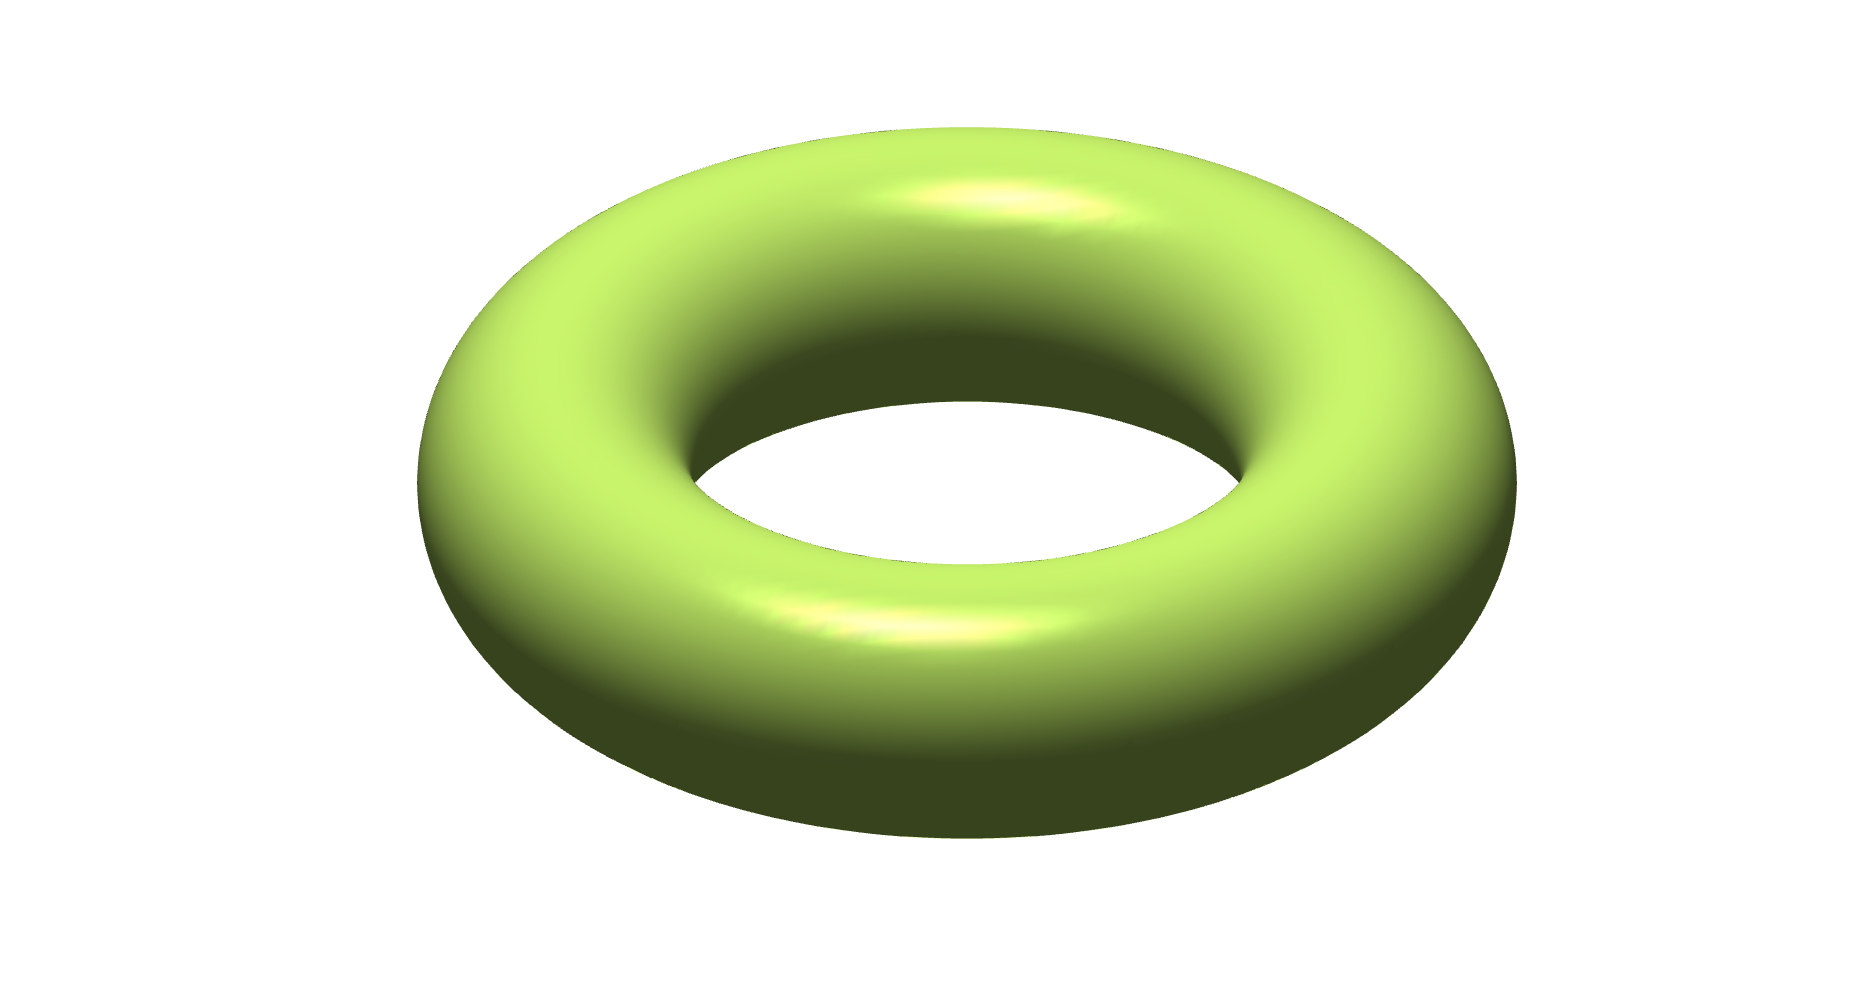
\includegraphics[width=0.21\columnwidth]{./img/torus}&
  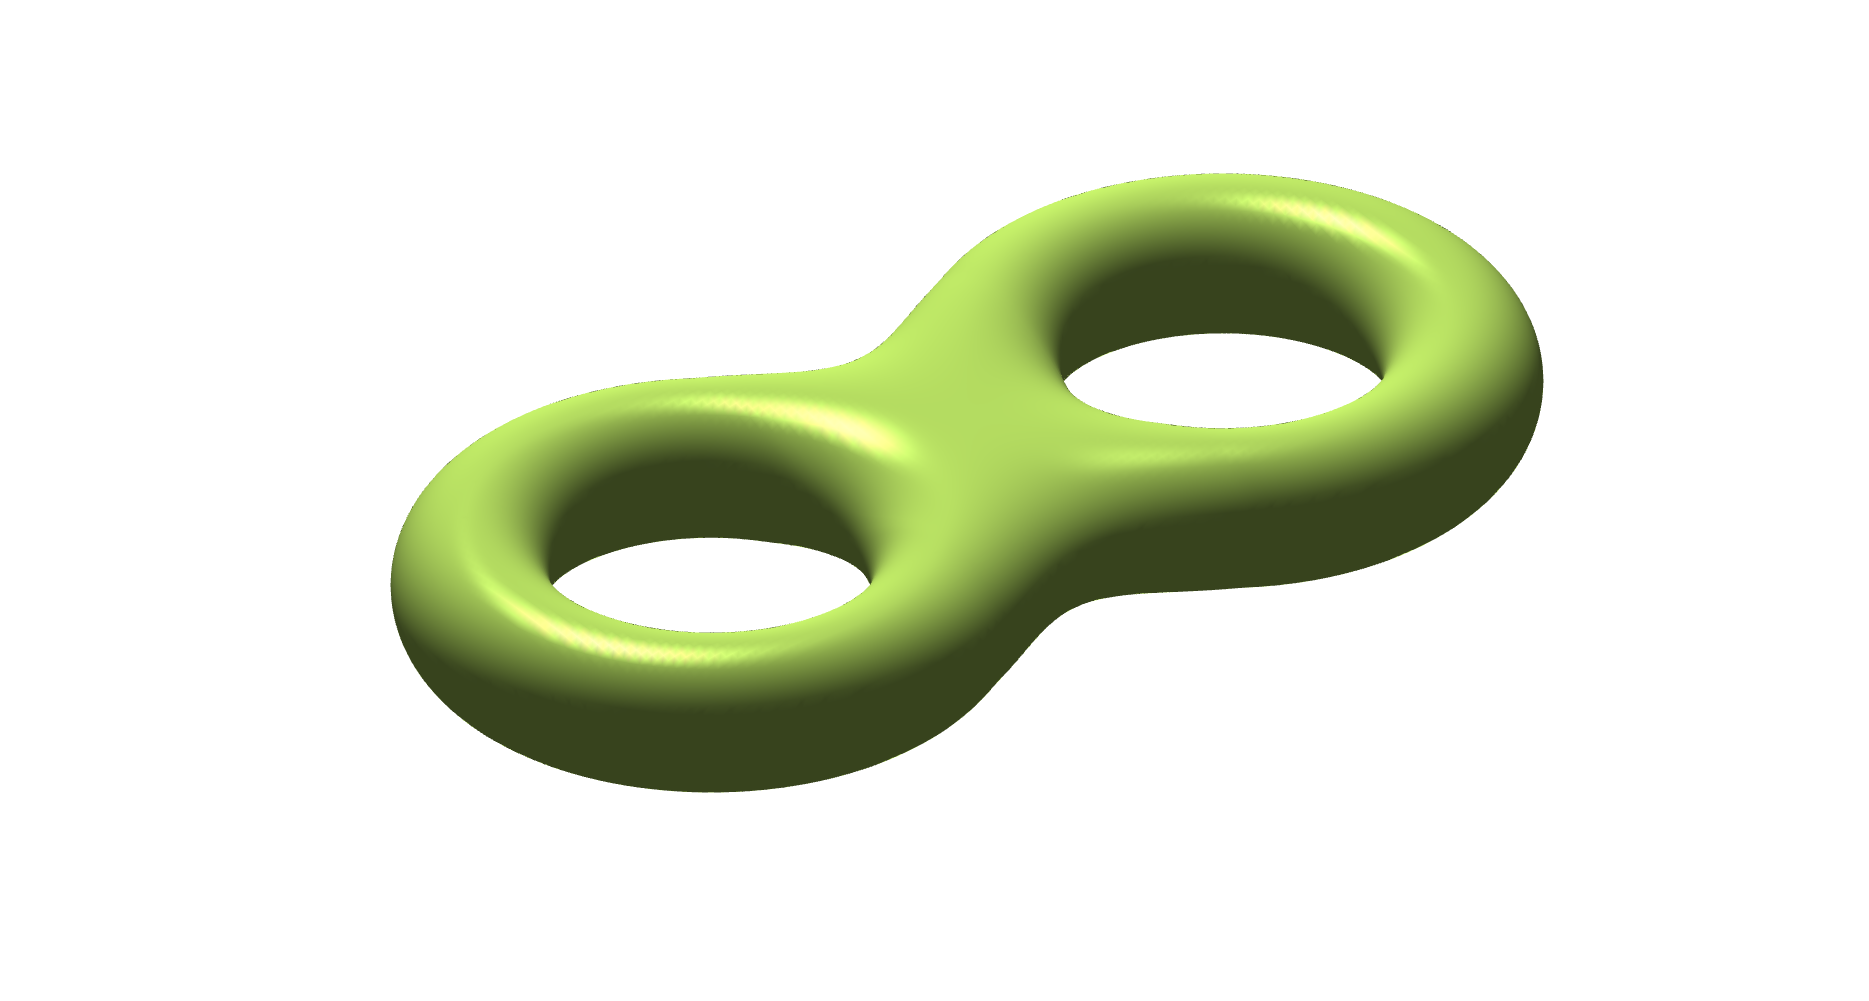
\includegraphics[width=0.21\columnwidth]{./img/doubleTorus}&
  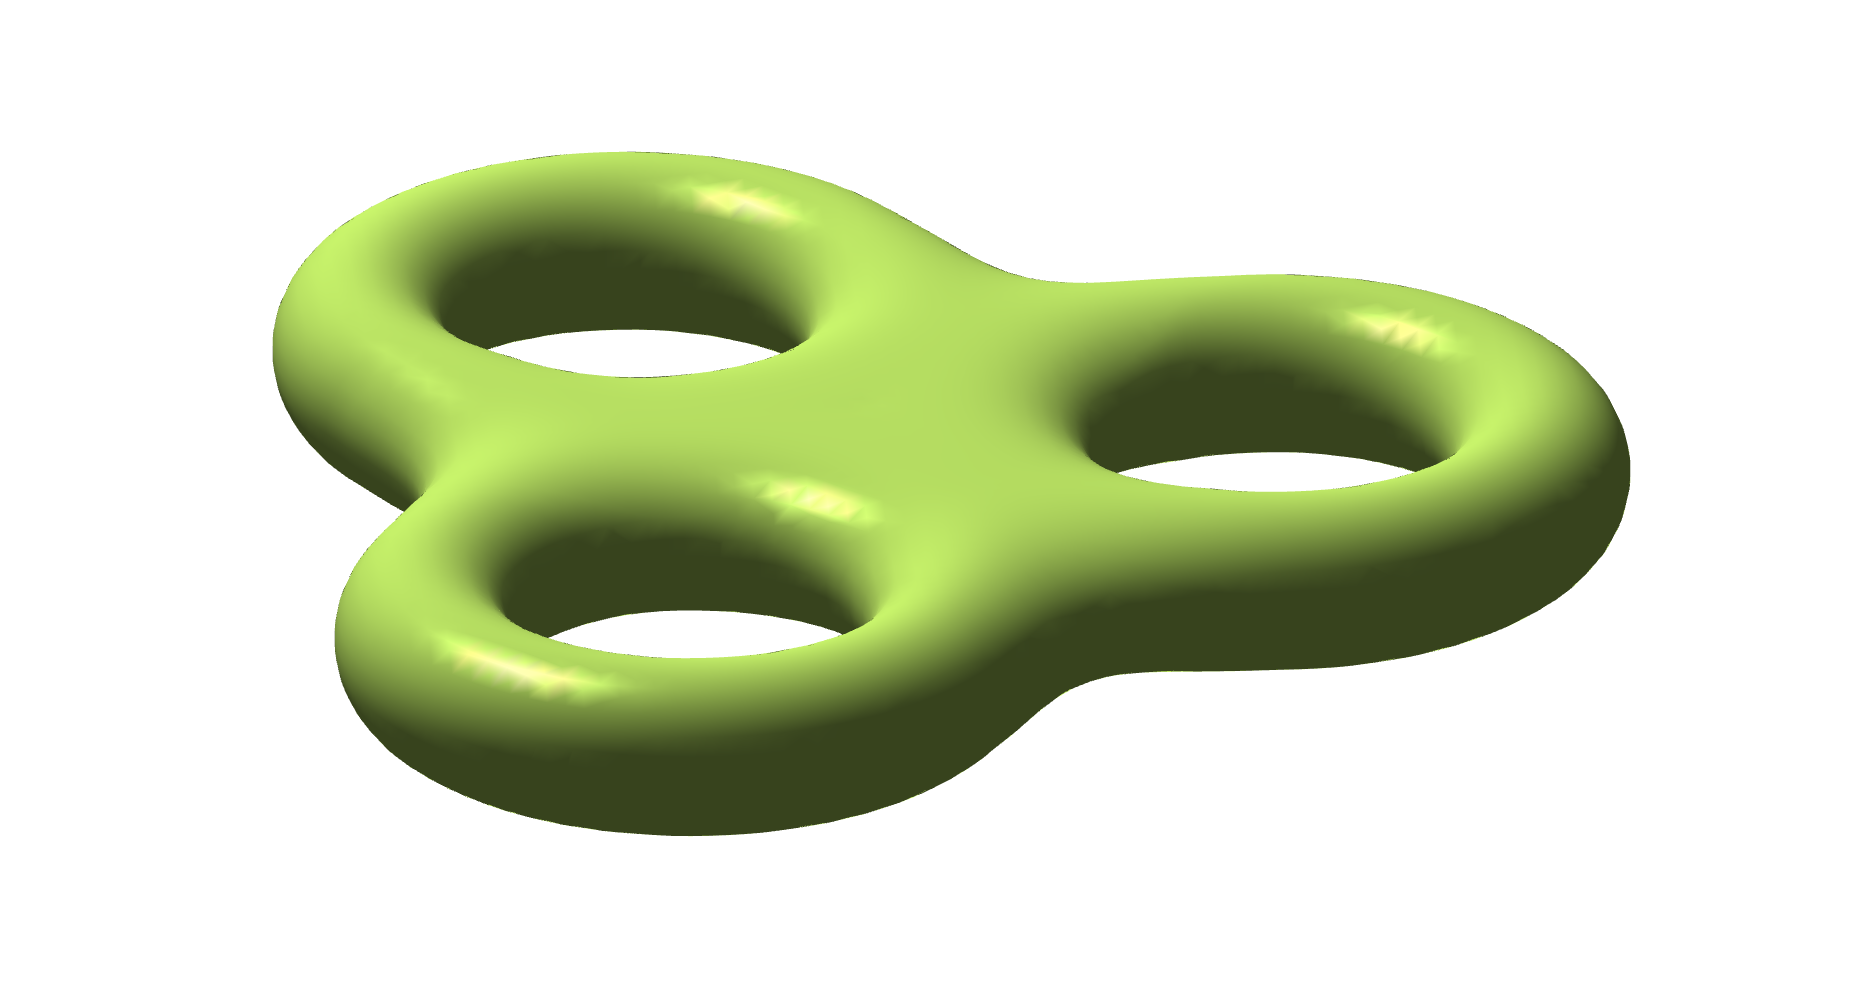
\includegraphics[width=0.21\columnwidth]{./img/tripletorus}\\
  Genus 0 & Genus 1 & Genus 2 & Genus 3
 \end{tabular}
 \caption{Example of surfaces with different genus.}
 \label{fig:torus}
\end{figure}



% \begin{thm}
% Here is a new definition
% \end{thm}

\section{Manifold Surfaces in the Discrete Domain}
The surface described thus far, can be discretized through the notion of a simplicial complex. 

Given $k + 1$ distinct points $v_0, \dots, v_k \in \mathbb{R}^n$, they are \emph{affinely independent} if a set of real numbers $\{c_0, \dots, c_k \}$ exists, such that the following equations:
\[
\sum_{i=0}^k{c_i v_i} = 0 \text{and} \sum_{i=0}^k{c_i} = 0
\]
are valid if and only if   $c_0 = \dots = c_k = 0$.


\begin{mydef}
 \textbf{$k$-simplex} 
 
 Let $\{v_0, \dots, v_k\}$ be a set of affinely independent points. The simplex spanned by this set of points is their convex hull
 \[
 \sigma = [v_0, \dots, v_k] = \left\{ \sum_{i=0}^{k}{t_i v_i} : t_i \geq 0 \text{and}  \sum_{i=0}^{k}{t_i} = 1\right\}.
 \]
\end{mydef}
In the previous relation, the values $t_i$ represent the barycentric coordinates and the each point in $\{v_0, \dots, v_k\}$ is named vertex.

Each simplex spanned by a nonempty subset of the vertices in $\sigma$ is called face, if $l\leq k$ is the cardinality of this subset, then is called $l$-face

The simplices in $\mathbb{R}^3$ are:
\begin{itemize}
  \item point: 0-simplex, with one 0-face;
  \item segment: 1-simplex, with two 0-faces and one 1-face;
  \item triangle: 2-simplex, with three 0-faces, three 1-faces and one 2-face
  \item tetrahedron: 3-simplex, with four 0-faces, six 1-facex, four 2-faces and one 3-face
\end{itemize}

\missingfigure{figure}


\begin{mydef}
\textbf{Simplicial complex}

A simplicial complex $C$ is a finite set of simplices satisfying two properties:
\begin{itemize}
  \item any face $\phi < \sigma$ of a simplex $\sigma \in C$ is also a simplex in $C$, i.e. $\phi \in C$
  \item if two simplices $\phi, \sigma \in C$, their intersection $\phi \cap \sigma$ is a face of both $\phi$ and $\sigma$
\end{itemize}
\end{mydef}
Some examples of simplicial complexes are the triangulations of a set of points in 2D, or the tetrahedrization in 3D.

\subsection{3D Delaunay Triangulation}
One of the most well-known 3D tetrahedrization, is the so called 3D Delaunay triangulation

\begin{mydef}
 \textbf{3D Delaunay Triangulation}
 Let $\mathit{P}$ be a set of $n \geq 4$ points in $\mathbf{R}^3$. A 3D Delaunay triangulation $T$ of $\mathit{P}$ is a 3-dimensional simplicial complex such that:
 \begin{itemize}
  \item $\mathit{P}$ is the set of vertices of T;
  \item the convex hull of $\mathit{P}$, is the union of the tetrahedra of $T$
  \item no vertex of $\mathit{P}$ is inside the circumscribing sphere of any tetrahedron of $T$.
 \end{itemize}

 
\end{mydef}

A 3D Delaunay triangulation always exists for $\mathit{P}$ and it is unique if  $\mathit{P}$ does not contain 5 cospherical points and does not contain 4 coplanar points.


Therefore, a 3D Delaunay triangulation $T$ is a particular set of tetrahedra whose vertices are the point in $\mathit{P}$; every tetrahedra has four neighbors, with except for the boundary tetrahedra $\delta T$, which have a facet with no neighbors. 
A common method to assign the missing neighbor to these tetrahedra, add a particular vertex $v_\infty$, named vertex at the infinity, connected to each of the boundary $\delta T$, such that virtual infinite tetrahedra are added to the triangulation $T$. 
This step enables a more coherent implementation of the Delaunay triangulation, by representing the tetrahedra and their neighboring relationships as a regular graph.

\subsubsection{Point addition and removal}
To implement an incremental reconstruction algorithm relying on the Delaunay Triangulation we will need to add points incrementally and possibly removing or moving them.

Whenever a new point has to be added into the triangulation  (the point B in Fig. \ref{fig:moving}(a)), a set of tetrahedra would conflict with it, i.e., the Delaunay property is not valid anymore (e.g., the light red triangles in Fig. \ref{fig:moving}(a)); so, this set of tetrahedra  is removed  (red triangles in Fig. \ref{fig:moving}(e)) and a new connected set that re-triangulate the hole is added to the triangulation(dark green triangles in Fig. \ref{fig:moving}(f)).

When a point has to be removed from the triangulation (e.g.,the point A in Fig. \ref{fig:moving}(a)), to keep the Delaunay property, all the tetrahedra incident to that point are removed (light red triangles in Fig. \ref{fig:moving}(b)); then,  a new set of tetrahedra is added and they  triangulate the resulting hole (dark green triangles in \ref{fig:moving}(c)).

Finally, the very common approach to deal with a point moving in the triangulation, is to remove it and add it back in the new position \cite{cgal} (Fig. \ref{fig:moving}): this process is therefore composed by the two procedures described above.

\begin{figure}[t]
\centering
\begin{tabular}{cccccc}
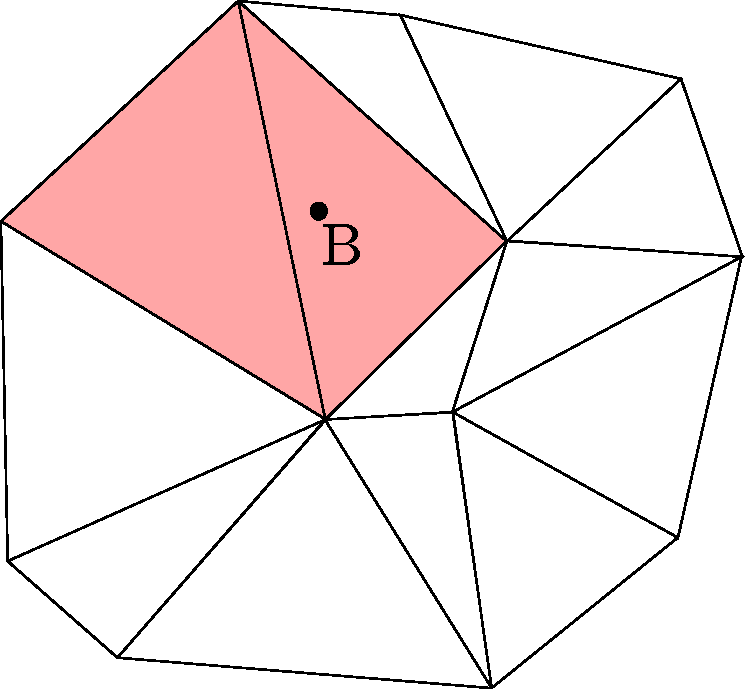
\includegraphics[width=0.25\columnwidth]{./img//delaunayExampleMoving04}&
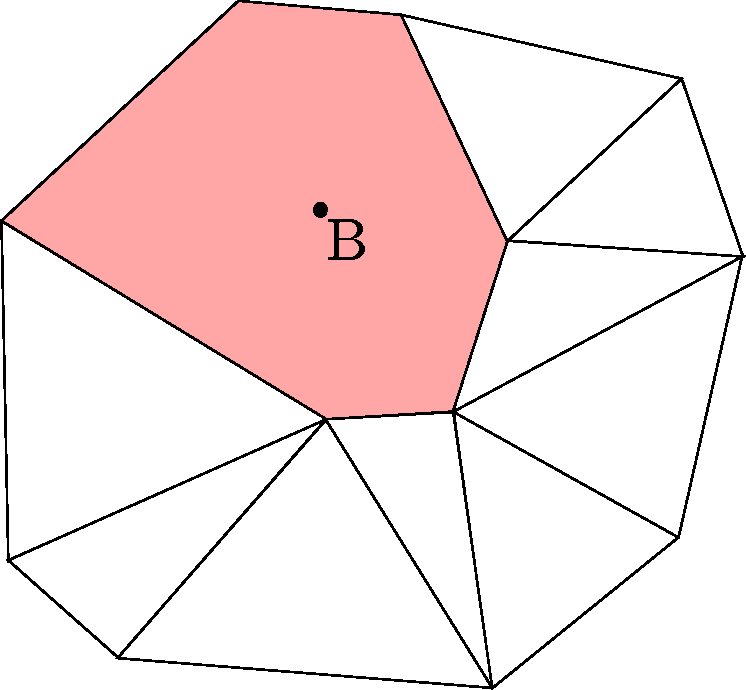
\includegraphics[width=0.25\columnwidth]{./img//delaunayExampleMoving05}&
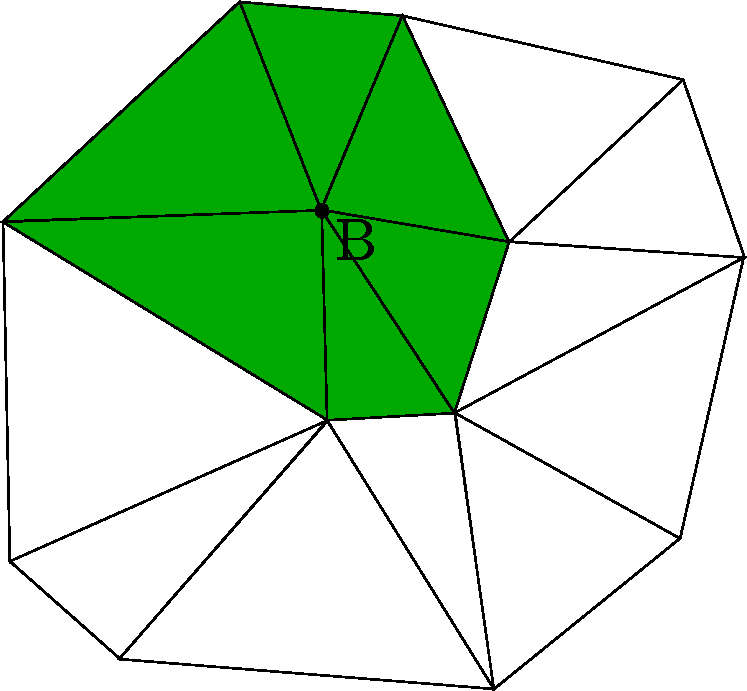
\includegraphics[width=0.25\columnwidth]{./img//delaunayExampleMoving06}\\
(a)&(b)&(c)\\
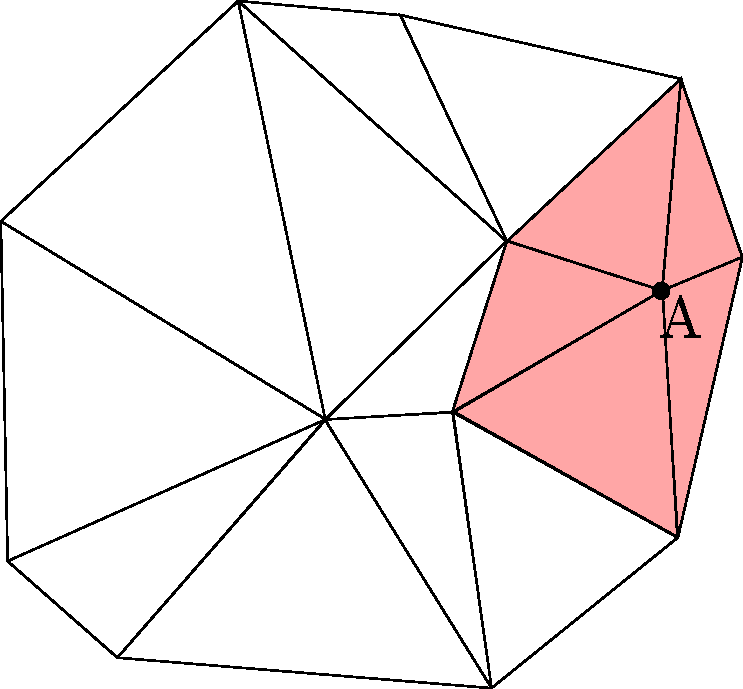
\includegraphics[width=0.25\columnwidth]{./img//delaunayExampleMoving01}&
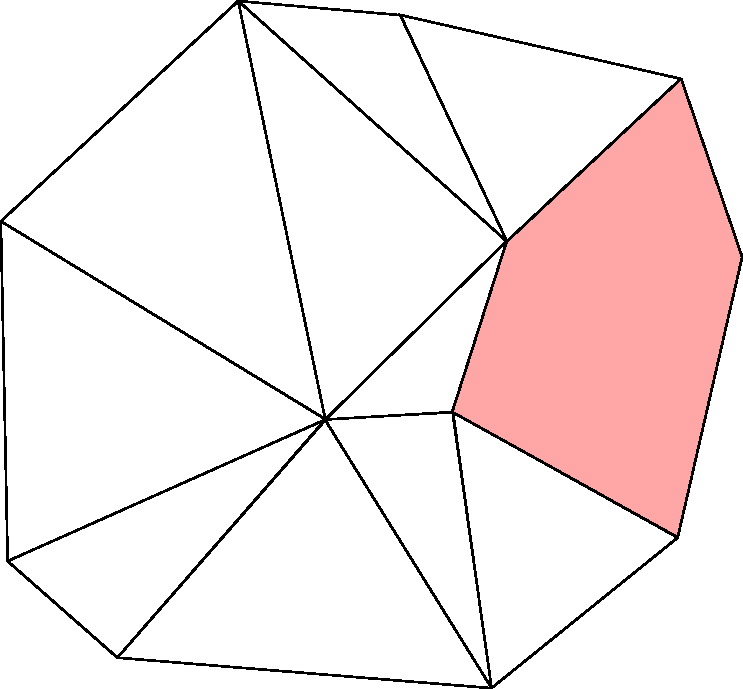
\includegraphics[width=0.25\columnwidth]{./img//delaunayExampleMoving02}&
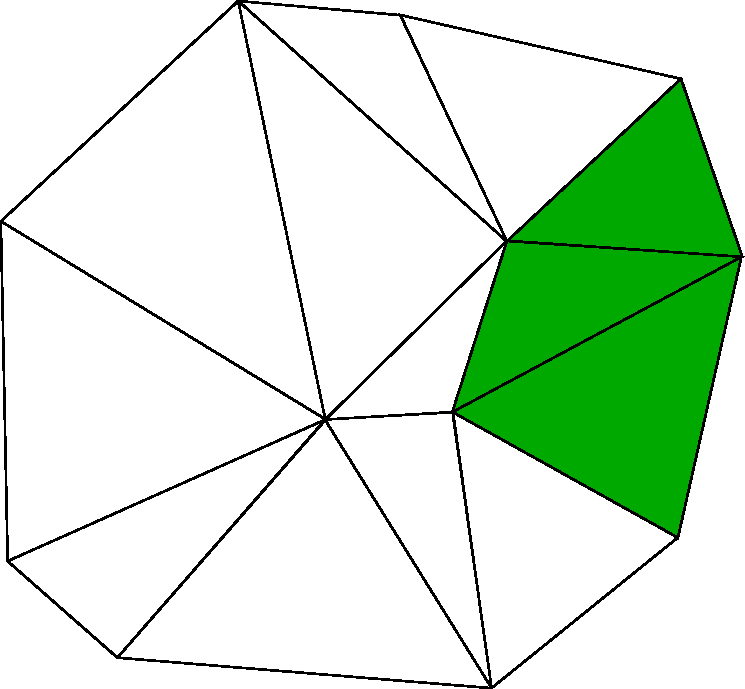
\includegraphics[width=0.25\columnwidth]{./img//delaunayExampleMoving03}\\
(d)&(e)&(f)
\end{tabular}
\caption{Point addition and removal in 2D case. Light red triangles depict removed and replaced with the new dark green ones.}
\label{fig:moving}
\end{figure}



\subsection{Manifold Tests}
In the first part of this thesis we aim at reconstructing the real world surface through a 2D simplicial subcomplex $\delta O$ of a Delaunay triangulation $T$ built upon a set $\mathit{P}$ of points belonging to the 3D surface.
In particular we look for a triangulated 2-manifold.

\begin{mydef}
\textbf{Triangulated $k$-manifold}

A triangulated $k$-manifold is a simplicial complex $\delta O$ such that the union of its simplices $|\delta O|$, named polyhedron, is $k$-manifold.
\end{mydef}

In our case $k=2$, and,in the following we use the term 2-manifold meaning triangulated 2-manifold.

To describe how to check if a $|\delta O|$ is 2-manifold, given a Delaunay triangulation $T$, we define a list $O$ of tetrahedra such that $O \subseteq T$. The simplicial complex $\delta O$ is the boundary of $O$, and we are able to check if the relative polyhedron is $k$-manifold through the tests described in \cite{lhuillier20152}.

First, we define the notion of good edges, and good vertex.


\begin{figure}
 \begin{tabular}{ccc}
  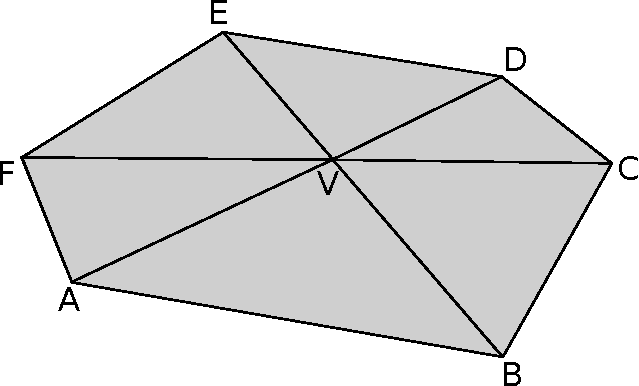
\includegraphics[width=0.3\columnwidth]{./img/manifold}&
  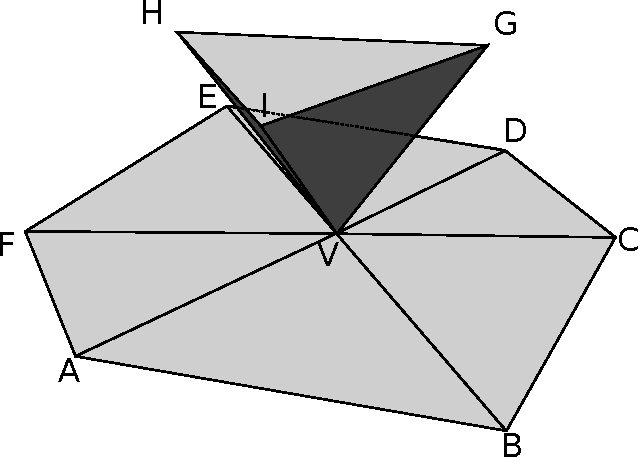
\includegraphics[width=0.3\columnwidth]{./img/notmanifold1}&
  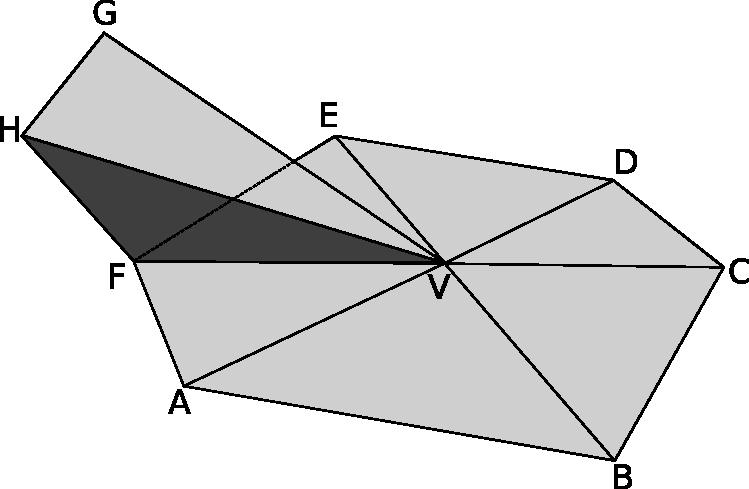
\includegraphics[width=0.3\columnwidth]{./img/notmanifold2}\\
  (a) & (b) & (c)
 \end{tabular}
 \caption{Example manifold (a) and non manifold surfaces (b) and (c).}
 \label{fig:manif}
 
\end{figure}



\begin{mydef}
\textbf{Good Edges}

An edge in $\delta O$ is a good edge if it is included in exactly two triangles of $\delta O$
\end{mydef}

For instance in Figure \ref{fig:manif}(a) the edge $AV$  is a good edge, is included in triangles $ABV$ and $AFV$; while in Figure \ref{fig:manif}(c) the edge $FV$ is not, since it is included in the triangles $ABV$, $AFV$, $FHV$ and $FGV$.

\begin{mydef}
\textbf{Good Vertex}

A vertex in $\delta O$  is a good vertex if the incident triangles in $\delta O$  can be ordered as
$t_0 , t_1, \dots, t_k$ such that $t_i \cap t_{(i+1) mod (k+1)}$ is an edge $\forall i \in {0, 1, \dots, k}$.
\end{mydef}

In Figure \ref{fig:manif}(a) the vertex $V$  is a good vertex (ordering of triangles: $ABV$, $BCV$, $CDV$, $DEV$, $EFV$ and $FAV$), while in Figure \ref{fig:manif}(b) the vertex $V$ is not (no ordering guarantee the above condition).

From these two, we are able to define the following test.

\begin{thm}
  \textbf{Global Test} 
  
  $|\delta O|$ is a 2-manifold if and only if contains only good vertices and good edges.
\end{thm}



A second, more practical and operational test is the following


\begin{thm}
  \textbf{Edge-Based Test} 
  
   A two-dimensional simplicial complex is a 2-manifold if and only if all the vertices are regular.
\end{thm}

where

\begin{mydef}
  \textbf{Regular vertex} 
  
   A vertex v is regular  if and only if the path of the opposite edges in the triangles having v as vertex is homeomorphic to a 2D disk.
\end{mydef}


For instance the vertex $V$ in Figure \ref{fig:manif}(a) is regular ($ABCDEF$ is a closed path and a single cycles, so is homeomorphic to a disk), while in Figure \ref{fig:manif}(b) and \ref{fig:manif}(c) the vertex $V$ is not regular since, in the former case the path $ABCDEFGHI$ is not closed, and in the latter $ABCDEFGHF$ has two cycles.


Finally we present a very useful manifold tests for incremental manifold reconstruction, proposed by \cite{litvinov_lhuillier_13}; by assuming $|\delta O|$ 2-manifold, the test aims at checking if the addition of one tetrahedron inside the list $O$, keeps the boundary $|\delta O|$ manifold.



\begin{thm}
  \textbf{One-tetrahedron addition test} 
  
  Assume that $|\delta O|$ is a 2-manifold. Let $\Delta \in T \setminus O$ and $(f,e,v)$ be a triplet representing respectively the number of triangles, edges, vertices in $ \Delta \cap \delta O$.
  $\delta (O \cup \{ \Delta \})$ is 2-manifold if and only if  $(f,e,v) \in  \{(0, 0, 0),\allowbreak (1, 3, 3),\allowbreak (2, 5, 4),\allowbreak (3, 6, 4),\allowbreak (4, 6, 4)\}$

\end{thm}
To better understand the triplets and the cases listed above see Figure \ref{fig:maniftest}, where the 

A similar test define if a tetrahedron subtraction keeps the manifold property valid (let note that subtracting $\Delta$ from $O$ is analogous to adding $\Delta$ to $T \setminus O$).


\begin{thm}
  \textbf{One-tetrahedron subtraction test} 
  
  Assume that $\delta O$ is a 2-manifold. Let $\Delta \in O$ and $(f,e,v)$ be a triplet representing respectively the number of triangles, edges, vertices in $ \Delta \cap \delta O$.
  $\delta (O \setminus \{ \Delta \})$ is 2-manifold if and only if  $(f,e,v) \in  \{(0, 0, 0),\allowbreak (1, 3, 3),\allowbreak (2, 5, 4),\allowbreak (3, 6, 4),\allowbreak (4, 6, 4)\}$
\end{thm}

\begin{figure}
 \begin{tabular}{ccccc}
  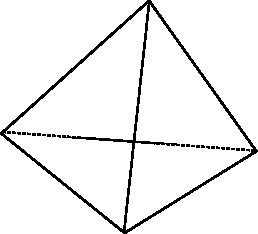
\includegraphics[width=0.15\textwidth]{./img/maniftest01}&
  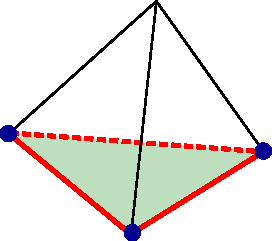
\includegraphics[width=0.15\textwidth]{./img/maniftest02}&
  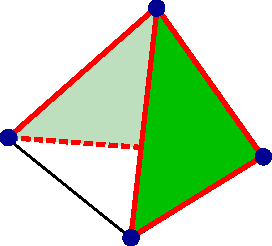
\includegraphics[width=0.15\textwidth]{./img/maniftest03}&
  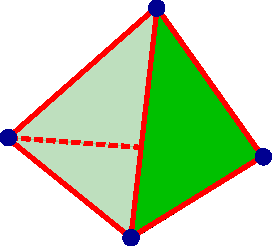
\includegraphics[width=0.15\textwidth]{./img/maniftest04}&
  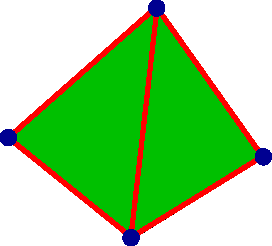
\includegraphics[width=0.15\textwidth]{./img/maniftest05}\\
  (0,0,0) & (1,3,3) & (2,5,4) & (4,6,3) & (6,6,4)
 \end{tabular}
 \caption{One Tetrahedron addition test: the figure depicts the five cases in of manifold-tetrahedron intersection that lead to a new manifold after tetrahedron addition; each triplets express the number of (vertices, edges, facets) in the intersection between the tetrahedron and the initial manifold.}
 \label{fig:maniftest}
 
\end{figure}

\section{Mesh processing}
One of the most common data structure in the computer graphics community is the so called triangle mesh \cite{botsch2010polygon}.

Intuitively a triangle mesh is a collection of 2D triangles, their edges and vertices in $\mathbb{R}^3$. 
These triangles represent a piecewise linear surface adopted to approximate a continuous real 3D surface. 

Formally, a triangle mesh $\mathit{M} = (V,E,F)$ is a simplicial complex with a set of vertices
\[
  \mathit{V} = \{v_1, \dots, v_V\}  
\]
a set of edges
\[
  \mathit{E} = \{e_1, \dots, e_E\}, \quad e_i \in \mathit{V}\times\mathit{V}
\]
and a set of faces
\[
  \mathit{F} = \{f_1, \dots, f_F\},\quad f_i \in \mathit{V}\times\mathit{V}\times\mathit{V}
\]

The geometric embedding of the simplicial complex $\mathit{M}$ in \Rthree is the homeomorphism $\mathit{P}$ that associates the vertices $v_i \in \mathit{V}$ with its position $p_i$:
\[
\mathit{P} = \{\mathbf{p_1}, \dots, \mathbf{p_v}\}, \quad \mathbf{p_i}:=p(v_i) = 
\begin{bmatrix}
x(v_i)\\
y(v_i)\\
z(v_i)
\end{bmatrix}
\in \mathbb{R}^3
\]
and associates each facet $f_i\in \mathit{F}$ to a triangle in \Rthree specified by the corresponding  3D vertices.
In the following, we make no distinction between the abstract elements of the simplicial complex and their actual embedding in the geometry of \Rthree.

A 2-manifold triangle mesh is a case of Triangulated $k$-manifold.

\subsection{Barycentric Coordinates}
Let $\mathit{t} = [\mathbf{a}, \mathbf{b}, \mathbf{c}]$ be a triangle; the position of every point $\mathbf{p} \in \mathit{t}$  can be expressed by the combination of the vertex positions:
\[
\mathbf{p} = \alpha \mathbf{a} + \beta \mathbf{b} + \gamma \mathbf{c}
\]
where 
\[
\alpha + \beta + \gamma = 1, \quad \alpha, \beta, \gamma \geq 0
\]
In Appendix \ref{app:barycentric_} we show how to compute these coordinates.

\subsection{Smoothing}
Mesh smoothing aims at estimating a smooth function $p$ defined on a triangular mesh.
Usually the function $p$ represent the position of the mesh vertices. 
Mesh smoothing can be approached as a signal analysis problem \cite{taubin1995signal}; the smoothing operation corresponds to the application of a low-pass filter.

In the continuous domain the Fourier transform is the common tool to design a low pass filter. 
The function $p(x)$ is transformed in $P(\omega)$ that is its representation in the frequencies domain:
\[
P(\omega) = \int_{-\infty}^{\infty} p(x) e^{2\pi i\omega x}dx.
\]
Now, we define the inner product among two functions $f$ and $g$, to prjoect the function $f$ in $g$ as:
\[
\langle f,g\rangle = \int_{-\infty}^{\infty} f(x) \overline{g(x)} dx
\]
where $\overline{g(x)}$ means the complex conjugate of $g(x)$, and the complex exponential function as:
\[
e_{\omega} := e^{2\pi i\omega x}.
\]
The function $p(x)$ can be written as follows:
\begin{equation}
p(x) = \sum_{\omega = -\infty}^{\infty} \langle p, e_{\omega}\rangle e_{\omega} = \sum_{\omega = -\infty}^{\infty} P(\omega) e_{\omega}.
\label{eq:continuousFourier}  
\end{equation}


A low-pas filter cuts the high frequency contributions in $p(x)$, therefore, by defining a cutting frequency $\omega_{max}$, the smoothed function $\widehat{p}(x)$ is:
\[
\widehat{p}(x) = \sum_{\omega = -\omega_{max}}^{\omega_{max}} \langle p, e_{\omega}\rangle  e_{\omega}.
\]

Since $e_{\omega}$ is an eigenfunction of the Laplacian operator $\bigtriangleup$:
\[
\bigtriangleup (e_{\omega}) = \bigtriangleup (e^{2\pi i\omega x}) = \frac{d^2}{dx^2}e^{2\pi i\omega x} = -(2\pi \omega)^2 e^{2\pi i\omega x}
\]
we obtain the analogous of \eqref{eq:continuousFourier} for a 3D discrete triangular mesh:
\[
\widehat{p}(x) = \sum_{\omega = 1}^{n} \langle p, \mathbf{e}_{\omega}\rangle  \mathbf{e}_{i}.
\]
where $\mathbf{e}_{i}$ are the eigenvectors of the Laplacian matrix $\mathbf{L}$ defined as:
\[
\label{eq:laplacianMatrix}
\begin{pmatrix}
  \bigtriangleup f(v_1)\\
  .\\
  .\\
  .\\
  \bigtriangleup f(v_n)
\end{pmatrix}
=
\mathbf{L}
\begin{pmatrix}
   f(v_1)\\
  .\\
  .\\
  .\\
   f(v_n)
\end{pmatrix}
\]
and the discrete Laplacian operator is:
\[
\label{eq:laplacian}
\bigtriangleup f(v_i) = \frac{1}{|\mathit{N(v_i)}|}\sum_{v_ \in \mathit{N(v_i)}} w_{ij} (f(v_j) - f(v_i)),
\]
with $\mathit{N(v_i)}$ corresponding to the set of neighboring vertices of $v_i$.
A more detailed descriptions are in \cite{botsch2010polygon,taubin1995signal,taubinygeometric,sorkine2005laplacian}.

Another approach to deal with the smoothing is the so called diffusion flow.
In the continuous case, let assume $f(\mathbf{x},t)$ be a function that evolves in time.
The evolution of this function is modeled as:
\[
\label{eq:continuousdiff}
\frac{\partial f(\mathbf{x},t)}{\partial t} = \lambda \bigtriangleup f(\mathbf{x}, t).
\]
This equation implies that the evolution of the function is proportional to its Laplacian $\bigtriangleup f$.

In the discrete case, we replace the continuous Laplacian operator, with the discrete Laplacian-Beltrami one, and we discretize by $h$ the time $t$ such that \eqref{eq:continuousdiff} becomes:
\[
\frac{\partial \mathbf{f}(t)}{\partial t} \approx \frac{\mathbf{f}(t+h) - \mathbf{f}(t)}{h}.
\]
and we obtain:
\[
\mathbf{f}(t+h) = \mathbf{f}(t) + h \lambda \mathbf{L}\mathbf{f}(t)
\]
where $\mathbf{L}$ is the Laplacian matrix in \eqref{eq:laplacianMatrix}.
As \cite{desbrun1999implicit} suggests, the implicit Euler integration leads to a solution more stable (numerically):
\[
\mathbf{f}(t+h) = \mathbf{f}(t) + h \lambda \mathbf{L}\mathbf{f}(t+h)
\]

When the function $\mathbf{f}$ represents the vertex positions, by applying the previous reasoning we are able to smooth the mesh geometry. In particular we update the vertices position $\{\mathbf{x}_1, \dots, \mathbf{x}_n\}$ by applying the so called \emph{Laplacian smoothing}:
\[
\mathbf{x}_i \leftarrow  \mathbf{x}_i  + h \lambda \bigtriangleup \mathbf{x}_i , \quad i = 1, \dots, n
\]
Different discrete Laplacian-Beltrami operators $\bigtriangleup$ exist \cite{wardetzky2007discrete,sorkine2005laplacian}, but the two most common are the uniform operator and the cotangent operator.

According to the definition in Eq. \eqref{eq:laplacian}, the weights of the uniform Laplacian operator, also known as umbrella operator, are 
\[
w_{ij} = 1 \quad iff \quad v_i and v_j \text{shares one edge}
\]
% \[
% \bigtriangleup f(v_i) = \sum_{v_ \in \mathit{N(v_i)}}(f(v_j) - f(v_i)),
% \]
i.e., this operator moves each vertex by averaging the positions of the neighboring.
The cotangent operator, also known as mean curvature flow operator, depends on the mesh geometry, and its weights are computed as:
\[
w_{ij} = \frac{1}{2} (cot(\alpha_{ij}) + cot(\beta_{ij})) \quad iff \quad \text{$v_i$ and $v_j$ shares one edge}
\]
where $\alpha$ and $\beta$ are those depitced in Figure \ref{fig:cotang}
\begin{figure}[t]
  \centering
  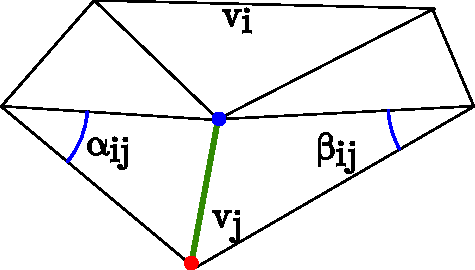
\includegraphics[width=0.7\columnwidth]{./img/laplacian}
  \caption{Cotangent laplacian operator terms.}
  \label{fig:cotang}
\end{figure}


% \[
% \bigtriangleup f(v_i) = \frac{1}{2A_i}\sum_{v_ \in \mathit{N(v_i)}} (cot(\alpha_{ij}) + cot(\beta_{ij})) (f(v_j) - f(v_i)),
% \]
%where $A_i$ is the averaging region, 
\subsection{Self Intersections}
When dealing with mesh evolution, the self intersection problem may arise. 
Ad Figure \ref{fig:selfint} show, when the vertices of the triangular mesh change their position sometime it happens  that a subset of triangles intersects another set of triangles, without sharing edges or vertices. 
In this case the geometrical entity created is no longer a simplicial complex, contains a sub-mesh not visible from the outside and the normals of this sub-mesh are not meaningful anymore.
For instance in Figure \ref{fig:selfint}(a) we show a silhouette of a mesh and the corresponding flow, which would induce the evolution of the mesh in Figure \ref{fig:selfint}(b), where the blue line underlines the self intersection.

The self intersections problem was faced by \cite{zara}.  
First, they find the self intersection by comparing each triangle against the triangles inside its bounding box, and extracting the segments $\mathbf{s}$ where two triangles intersect. 
Then, they look for one external facet $f_{\text{init}}$, they add it to a set $\mathit{T}$, and from $f_{\text{init}}$ they collect the adjacent triangles in $\mathit{T}$, by checking them as viseited, till they reach the triangles containing the self intersections $\mathbf{s}$, which are stored in the set $\mathit{S}$.  
For each triangle in $\mathit{S}$ and the corresponding self intersection segment $\mathbf{s}$, they perform a constrained 2D Delaunay triangulation on their plane, and add the resulting triangle to $\mathit{T}$.
They continue these steps until no more triangle facet has to be visited.
Finally,  they compute the final mesh by stitching together the triangles in $\mathit{T}$.

\begin{figure}
 \begin{tabular}{cc}
  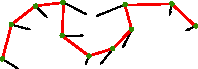
\includegraphics[width=0.45\textwidth]{./img/selfinters01}&
  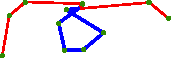
\includegraphics[width=0.45\textwidth]{./img/selfinters02}\\
  (a)&(b)
 \end{tabular}
 \caption{Example of self-intersection: a mesh evolves according to the vector flow illustrated in (a); the outcome (b) is a self-intersecting mesh (blue lines).}
 \label{fig:selfint}
\end{figure}

\subsection{Mesh subdivision}
A very common and useful operation on meshes is named mesh subdivision, whose input is a mesh, named control mesh, and outputs a mesh geometrically refined and eventually smoothed. I
New vertices are computed for each edge (edge point), facet (facet point) and vertex (new point) of the control mesh, by averaging a, usually very small subset of neighboring vertices.


Several algorithm was proposed, and they differs on how the vertices of the new mesh are computed. 
The most common methods are: , Catmull-Clark \cite{catmull1978recursively}, Doo-Sabin \cite{doo1978subdivision} and Loop.

\subsubsection{One-to-four midpoint}

This is the simplest method to subdivide a control mesh for triangular meshes: it does not smooth the resulting mesh, but it just subdivide each triangular facet in four triangles such that it preserves the edges of the control mesh.
In this simple subdivision method no facet point are computed; the edge points are in the midpoint of each edge and the new vertex position coincides with the old vertec position.


In Figure \ref{s} we show how this subdivision scheme acts on a single facet.


\subsubsection{Catmull-Clark}
The Catmull-Clark subdivision scheme adds a new points and facets, and moves the vortices of the control mesh. 
For each facet $f_i$, a new face-point $fp_i$ is added in the average position of the corresponding polygon vertices. 
For each edge $e_i$, it takes into account the adjoint facets $f_{ik}$ and $f_{ih}$ and creates a new vertex (edge-point) in the average position of the mid point of the edge $e_i$, and the facet-points $fp_{ik}$ and $fp_{ih}$ corresponding to $f_{ih}$ and $f_{ih}$.
Then, it moves each old vertex $v_i$ in position $V$ in a new position:
\[
p(v_i^{\text{new}}) = \frac{(n-3)V + 2E + FP}{n}
\]
where $E$ represents the average position of the edges incident to $v_i$ and  $FP$ is the average position of the facet-points corresponding to the $n$ facets incident to $v_i$.

Finally, the new points are connected as follows: each face point to an edge point, which connects to a new vertex point, which, in turn, connects to the edge point of the adjoining edge, which returns to the face point.


\subsubsection{Loop}
The Loop scheme takes as input a triangular mesh and subdivide each triangular facet in four new smaller triangles, analogously to the one-to four scheme.
Instead of choosing the mid point as the edge point, for each edge $e_i = v_av_b$ it computes each edge point taking into account the adjoint facets $f_{ik} = v_av_bv_k$ and $f_{ih}v_av_bv_h$ and the position of the edge point $ep_i$ is computed as:
\[
ep_i = \frac{3(p(v_a) + p(v_b)) + (p(v_k) + p(v_h)) }{8}.
\]

Then the position of new vertex points $v_i^{\text{new}}$ are computed from the position of the old vertex and the $n$ neighboring vertices $v_j^{\text{neig}}, j = 1,\dots, n$ as:
\[
(1-s) n v_i + s \sum_{j=1}^n v_j^{\text{neig}}
\]
where, the scaling factor $s$ is:
\[
s=
\begin{cases}
  3/16 \qquad \text{if $n = 3$}\\
  \frac{1}{n} \left(\frac{5}{8} - \left(\frac{3}{8} + \frac{1}{4} cos\left(\frac{2\pi}{n}\right)\right)^2\right) \qquad \text{if $n > 3$}
\end{cases}
.
\]

No facet point are computed.

\subsubsection{Doo-Sabin}

The Doo-Sabin subdivision method, as the Catmull-Clark, applies on both triangular and quadrilateral meshes.

The edge points are computed as the midpoint of each edge. 
The facet points are the correpsonding centroid. 
For each vertex $v_i$, the new vertex points is computed as the average of the position of $v_i$ and the facet points computed from the facets incident in $v_i$ and the edge points computed from the edges incident to $v_i$.

Finally, the following procedure creates the new mesh. 
For each old facet, connect the new points generated inside the facet itself.
Then, for each vertex, connect the face points generated from the faces that are adjacent to this vertex. 
And for each edge, connect the new face points generated from the faces adjoining to this edge. 




The CGAL library provide a package \cite{cgal:s-ssm2-15b} to fully manage the subdivision process on manifold meshes.



